
\begin{figure}
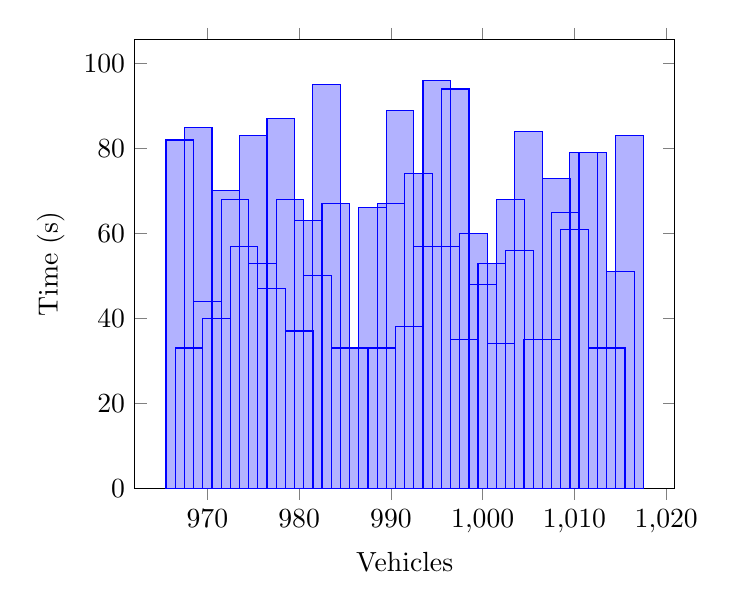
\begin{tikzpicture}
\begin{axis}[
legend style={anchor=west},
xlabel=Vehicles,
ylabel=Time (s),
ymin=0,
ybar,
]
\addplot coordinates {
(1004, 56)
(990, 67)
(986, 33)
(1014, 33)
(970, 44)
(1000, 48)
(978, 87)
(995, 96)
(974, 57)
(994, 57)
(980, 37)
(1013, 33)
(972, 70)
(991, 89)
(1012, 79)
(1008, 73)
(975, 83)
(1003, 68)
(997, 94)
(1007, 35)
(1006, 35)
(993, 74)
(967, 82)
(971, 40)
(968, 33)
(981, 63)
(996, 57)
(977, 47)
(1010, 61)
(1009, 65)
(989, 33)
(1016, 83)
(976, 53)
(1005, 84)
(979, 68)
(998, 35)
(1001, 53)
(992, 38)
(983, 95)
(988, 66)
(969, 85)
(987, 33)
(985, 33)
(1011, 79)
(984, 67)
(1002, 34)
(999, 60)
(1015, 51)
(973, 68)
(982, 50)
};

\end{axis}
\end{tikzpicture}
\label{tik:time:0:89}
\caption{0 percent diving with GSC on route $89$}
\end{figure}
